% don't use 'we' from instead use passive
\documentclass[a4paper]{jpconf}
%\bibliographystyle{iopart-num}
%\usepackage{citesort}
\usepackage{listings}
\usepackage{graphicx}

%basicstyle=\ttfamily \scriptsize,    % the size of the fonts that are used for the code \footnotsize
\lstset{ % General settings
language=,                   % choose the language of the code
basicstyle= \sffamily \scriptsize,        % the size of the fonts that are used for the code \footnotsize
showspaces=false,               % show spaces adding particular underscores
showstringspaces=false,         % underline spaces within strings
showtabs=false,                 % show tabs within strings adding particular underscores
frame=,                         % adds a frame around the code (single)
tabsize=2,                      % sets default tabsize to 2 spaces
captionpos=t,                   % sets the caption-position: top (t), bottom (b)
breaklines=true,                % sets automatic line breaking
breakatwhitespace=false,        % sets if automatic breaks should only happen at whitespace
escapeinside={\%*}{*)},         % if you want to add a comment within your co>de
caption=footnote, 
label=listing:relRef
}

\newcommand{\Hplustaunu}{\mbox{${\rm H}^{\pm} \to \tau^{\pm}\nu_{\tau}$}}
\newcommand{\pT}{\mbox{${\rm p}_{\rm T}$}}

\begin{document}
\title{Ideal $\tau$ tagging with TMVA multivariate data-analysis toolkit}

\author{A Heikkinen, P Kaitaniemi, V Karim\"{a}ki,
M~J Kortelainen, T~Lamp\'{e}n, S Lehti, T Lind\'{e}n and L Wendland} 

\address{Helsinki Institute of Physics, P.O. Box 64, FIN-00014 University of Helsinki, Finland}

\ead{aatos.heikkinen@cern.ch}


\begin{abstract}
The experience on using ROOT package TMVA for
multivariate data analysis is reported for a problem of $\tau$ tagging in the
framework of heavy charged MSSM Higgs boson searches at the LHC.
With a generator level analysis,
we investigate how in the ideal case $\tau$ tagging could be performed and
hadronic $\tau$ decays separated from the
hadronic jets of QCD multi-jet background present in LHC experiments.
A successful separation of the Higgs signal from the background
requires a rejection factor of $10^5$ or better against the QCD background.
The $\tau$ tagging efficiency and background rejection are studied with various MVA classifiers.
\end{abstract}


\section{Introduction}
Multivariate analysis methods have rapidly become important in high energy physics.
The rare and subtle signals are hidden within voluminous data, 
and their analysis calls for multivariate algorithms, since taking
full correlations into account can greatly increase the ability to separate signal
from background~\cite{statlearn}.


The ROOT package TMVA for multivariate data analysis was previously demonstrated
to be usable to b-tagging~\cite{chep07tmva}. In this study, the TMVA
package is applied to $\tau$ identification in the heavy charged MSSM Higgs
boson decay \Hplustaunu~$\to {\rm hadrons}$. In previous studies
conducted in the CMS experiment, this channel has been found to
provide an interesting possibility do discover the charged Higgs
boson~\cite{ptdrII}, should it exist.

The challenge of this physics channel is, that the cross-section of
the largest background, i.e. QCD multi-jets, which could fake
hadronically decaying $\tau$'s, is up to 10$^7$ times
greater than the signal cross-section at the 14~TeV center of mass
collision energy of the LHC. 
Since the production of such large Monte Carlo samples is not
currently feasible with full detector simulation, generator level
simulation was used to obtain an estimate for the
benefit of the use of multivariate methods to separate the signal and
background.

It is estimated, that a rejection factor of 10$^{-5}$ is needed with
$\tau$ identification in order to make the charged Higgs boson signal
visible~\cite{ptdrII}. Therefore, the performance of the selected MVA
classifiers was evaluated for background rejection of 10$^{-5}$ and
10$^{-6}$. Moderate customisation was required to map the study into
the TMVA framework.

This article is organised as follows. Section~\ref{sec:tmva} introduces
TMVA toolkit for parallel multivariate data analysis,
Section~\ref{sec:data} describes the Monte Carlo data prepared for this study,
Section~\ref{sec:customization} outlines a customization of TMVA for $\tau$ tagging,
and Section~\ref{sec:results} gives results using various TMVA discriminators.

\section{TMVA - Toolkit for Parallel Multivariate Data Analysis}\label{sec:tmva}

ROOT-integrated TMVA is a framework the training, testing and performance evaluation
of multivariate classification techniques.
TMVA works in transparent factory mode 
to guarantee an unbiased performance comparison between the classifiers, such as:

\begin{itemize}
\item Rectangular cut optimisation
\item Projective likelihood estimation (PDE approach)
\item Multidimensional probability density estimation (PDE - range-search approach, PDERS)
\item Multidimensional k-nearest neighbour classifier
\item Function discriminant analysis (FDA)
\item Predictive learning via rule ensembles (RuleFit)
\end{itemize}
 
Main characteristics of different TMVA classifiers are summarised in Table~\ref{tab:characteristics}.

\begin{center}
\begin{table}[h]
\footnotesize
\caption{\label{tab:characteristics} Main characteristics of different
classifiers~\cite{tmvaPhystat}.}
%\footnotesize\rm
\centering
%\begin{tabular}{@{}*{7}{l}}
\begin{tabular}{lll}
\br
Method & Pros & Cons\\
\mr
Cuts & Easy to understand & Possibly inefficient \\
Likelihood methods & Fast to train and evaluate & Non-linear
correlations treated badly \\
HMatrix, Fisher & Very fast and transparent & fail if PDFs have same
mean,\\
      &                           & and if non-linear correlations\\
PDERS, kNN & Handles well complex class boundaries & Impractical with more
than 10 variables\\
ANN & Very good with non-linear correlations & Black box, needs tuning\\
BDT & Very good out-of-the-box performance & Needs tuning to avoid
overtraining \\
RuleFit & Like BDT but simpler, fast evaluation & Often needs some
tuning\\
SVM & Good with non-linear problems,   & Not
transparent\\
   &          insensitive to overtraining &  \\
FDA & Very good classification if boundary is known & Classification
boundary function needed\\
\br
\end{tabular}
\end{table}
\normalsize
\end{center}

\vspace{0.5cm}
The following MVA methods were selected for evaluating the TMVA performance:
\begin{itemize}
\item Linear discriminant analysis (LDA) based on Fisher discriminants
\item Boosted/Bagged decision trees (BDT)
\item Support Vector Machine (SVM) 
\item Artificial neural networks (ANN)
\end{itemize}


\section{Data}\label{sec:data}
The signal was generated with Pythia~\cite{pythia} version 6.4.19
through the process ${\rm gg} \to {\rm tbH^\pm}$,
\Hplustaunu\ in the maximal 
${\rm m}_{\rm H}$ SUSY scenario~\cite{maxsusy} with 
${\rm m}_{{\rm H}^{\pm}}=217~{\rm GeV/c}^2$ and $\tan\beta = 30$.
The $\tau$ leptons were forced to decay hadronically. The decay of the
$\tau$ leptons was simulated with the Tauola program~\cite{tauola}
version 2.6 to obtain correct polarization for the $\tau$ lepton and
its decay products~\cite{taupolarization}. $10^5$ and $2\times 10^5$
signal events were produced for training and evaluation of the
multivariate analyzers, respectively.

The dominating background for this physics channel is the QCD
multi-jet background. This background was generated with 
Pythia version 8.108. The transverse momentum of the hadronic jets was
limited to the bin $120 < \hat{\rm p}_{\rm T} < 170$~GeV/$c$, which
has been found to be the most difficult $\hat{\rm p}_{\rm T}$
range~\cite{ptdrII}. Training and evaluation samples of $5\times 10^6$
and $10^8$ QCD multi-jet events were produced respectively. Another
independent sample of $5\times 10^6$ events was used as a second
training sample to estimate the bias caused by the training.

The events were generated with p-p collisions at center of mass energy
of 14~TeV. The jets were reconstructed with the PYCELL-method in a
cone of 0.5 in $(\eta$,$\phi)$ space. For the signal, only the jets
corresponding to the $\tau$ decay, i.e. $\tau$ jets were taken as
$\tau$-jet candidates. For the background events, all jets obtained
with PYCELL-methods were taken as $\tau$-jet candidates.

%\subsection{Production and Preselection Cuts}
In order to save CPU time and disk space, a set of preselection cuts
was applied to the $\tau$-jet candidates. These are standard cuts,
which are used for $\tau$ identification~\cite{tautagging}. Care was
taken, that the preselection cuts were loose enough in order not to
bias the MVA performance. The following preselections were used:
\begin{itemize}
\item jet ${\rm E}_{\rm T} >$ 100 (Fig.~\ref{fig:variables})
\item jet $|\eta|<$~2.2 
\item the leading track, i.e. the track with the highest \pT, within a
  cone of 0.1 of the jet direction in $(\eta$,$\phi)$ space
\item cut on the \pT\ of the leading track, \pT~$>$~20~GeV/$c$
\item $\eta$ of tracks, $|\eta|<$~2.5
\item minimum \pT\ of charged tracks,
  ${\rm p}_{\rm T}^{\rm min} >$~0.5~GeV/$c$
\item track matching to primary vertex along the beam axis, $|{\rm
  IP}_{\rm z}^{\rm track}-z|<2$~mm
\item one or two tracks in a signal cone size of 0.04 in $(\eta$,$\phi)$
  space around the leading track
\item zero or one tracks in an isolation annulus between the signal
  cone and a cone of 0.5 in $(\eta$,$\phi)$ space around the leading track 
\end{itemize} 
The preselection efficiencies were found to be ??? and ??? for the
signal and background samples used for the evaluation of the MVA
methods, respectively.

The number of tracks in the signal cone of 0.04 in $(\eta$,$\phi)$ space
around the leading track was set as one in order to select the
one-prong final state of $\tau$ decays, which is dominant of the
hadronic $\tau$ decay final states.
Of variables, which are standardly used for $\tau$ idenfitication in
the \Hplustaunu\ decay, the most important ones were used as input to
the MVA methods.
These variables include a cut on the transverse energy and
pseudo-rapidity of the $\tau$-jet candidate, maximum track \pT\ in the
isolation annulus between cones of 0.04 and 0.50 around the leading
track direction in $(\eta$,$\phi)$ space to impose charged track
isolation, sum of electromagnetic energy in the region between cones
of 0.10 and 0.50 around the jet axis in $(\eta$,$\phi)$ space and
matching of the hadronic energy deposition to the leading track
momentum to reject electrons~\cite{tautagging}. Furthermore, the 
${\rm R}_\tau = {\rm p}_{\rm track} / {\rm E}_{\tau}$ variable, where 
${\rm E}_{\tau}$ is the reconstructed $\tau$-jet candidate energy
(excl. neutrinoes), was used to take advantage of the boost of the
$\tau$ due to polarization~\cite{taupolarization}.
The variables are summarized in Table~\ref{tab:variables}.
Figure~\ref{fig:variables} shows
the distributions of the jet ${\rm E}_{\rm T}$ and ${\rm R}_\tau$
variables, which were found to have the best separation
power. The input variables were used without transformations as well
as with decorrelation or principal component analysis applied.

\begin{table}[h]
\begin{center}
\caption{\label{tab:variables}Variables used in the analysis.}
\begin{tabular}{l*{2}{l}r}
%\hline
\br
ID & Variable                                                       \\
%\hline
\mr
0 & Jet ${\rm E}_{\rm T}$                                        \\
1 & Jet $\eta$                                                   \\
2 & Charged track isolation in annulus                           \\
3 & Isolation of electromagnetic energy ($\Delta$R=0.10 - 0.50)  \\   
4 & Neutral hadron rejection                                     \\
  & (i.e. track p matching to hadronic energy deposition)        \\
5 & ${\rm R}_{\tau}$ = p(leading track) / E(jet)                 \\
%\hline
\br
\end{tabular}
\end{center}
\end{table}



\begin{figure}[h]
 \begin{minipage}{7.8cm}
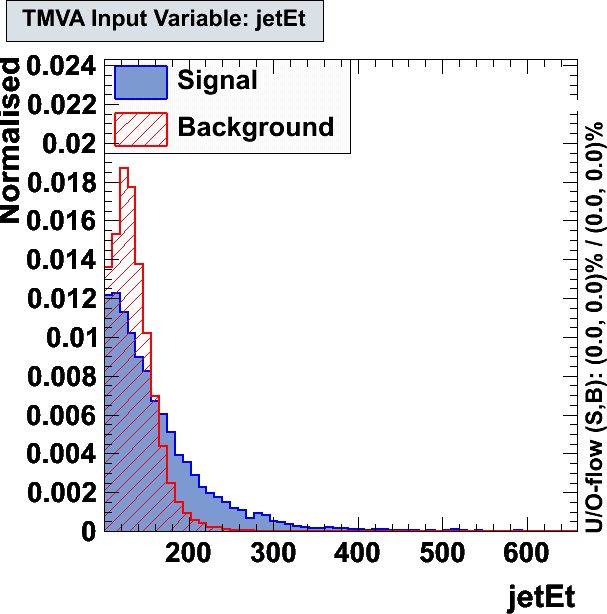
\includegraphics[width=0.9\textwidth]{images/jetet.png}
\end{minipage}
 \hfill
\begin{minipage}{7.8cm}
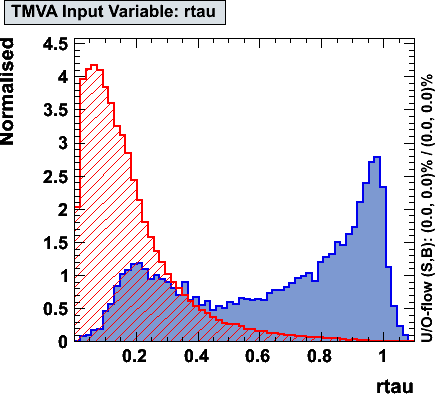
\includegraphics[width=1.0\textwidth]{images/rtau.png}
\end{minipage}
%\begin{minipage}{3.0cm}

\caption{Example of data used in $\tau$ tagging.
Distributions of jet ${\rm E}_{\rm T}$ and ${\rm R}_{\tau}$  variables are shown.}
%\end{minipage}
\label{fig:variables}
\end{figure}


%\begin{center}
%\begin{table}[h]
%\caption{\label{opt}Summary of {\sf QGSP\_\-INCL\_ABLA} physics list.}
%\footnotesize\rm
%\centering
%\begin{tabular}{@{}*{7}{l}}
%\br
%Option&Description\\
%\mr
%\verb"Al-"&Targets heavier than Aluminium.\\
%\verb"150~MeV -"&Projectile energies from $\sim$ 150 MeV up to 2.5 GeV $\sim$ 3 GeV.\\
%\br
%\end{tabular}
%\label{tab:}
%\end{table}
%\end{center}





%{\sf QGSP\_\-INCL\_ABLA} with

 
%\begin{figure}[h]
% \begin{minipage}{7.0cm}
%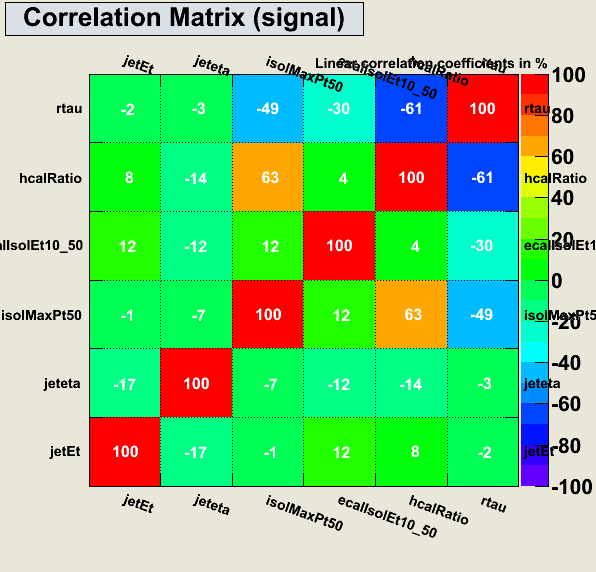
\includegraphics[width=1.0\textwidth]{images/ahCorrelationMatrixS.png}
%\end{minipage}
% \hfill
%\begin{minipage}{7.0cm}
%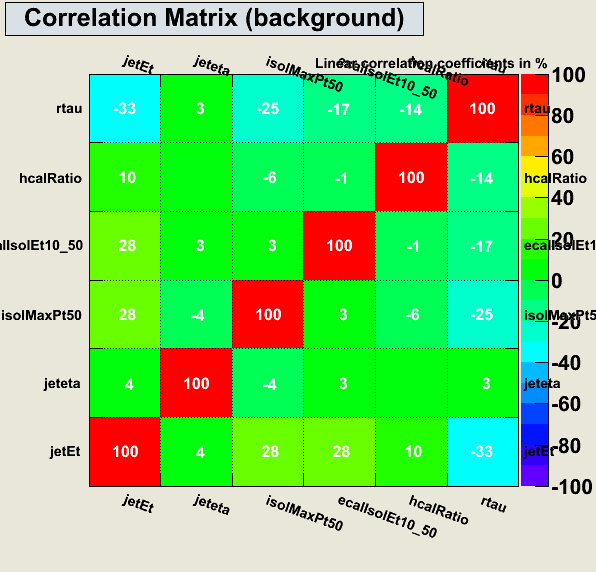
\includegraphics[width=1.0\textwidth]{images/ahCorrelationMatrixB.png}
%\end{minipage}
%\begin{minipage}{3.0cm}
%\caption{Right: Variable correlation matrix for signal Right: Variable correlation matrix for background}
%\end{minipage}
%\label{fig:ahCorrelationMatrix}
%\end{figure}

\section{Customization of TMVA for $\tau$ tagging}\label{sec:customization}
Since the performance of the MVA methods was to be evaluated at a
background rejection 10$^{-5}$ and 10$^{-6}$, the TMVA package had to
be customized slightly for the analysis.
Firstly, since the root trees contained jets, and since a single event
could contain several jets, a functionality to evaluate the $\tau$
identification efficiency calculated per event was added to  {\tt TMVA::Reader}.  
Customization was made to TMVA distributed with ROOT 5.21/06.


The algorithm is described in pseudocode in
Appendix~A. %Listing~\ref{listing:eventcode}.
The algorithm had to take into account also the preselection
efficiencies of the event samples used for evaluation. Additionally,
timing profiling with {\tt TStopwatch} was added.

Also the evaluation of the signal efficiency at high background rejection
level required some customization.

[describe here in more detail what was done]

% what is the point of the following sentence? please clarify
Example Listing~\ref{listing:log} in Appendix A from analysis run demonstrates these customisations.


\section{Results}\label{sec:results}

\subsection{Classifying with Fisher discriminant}
The method of Fisher discriminants is a computationally easy method,
which determines the discriminating function analytically in the
multivariate space represented by the input variables.  It has been
used in analyses of several HEP experiments, for instance in BaBar \cite{fisherbabar} and
Belle \cite{fisherbelle}

The Fisher method works in a transformed variable space with zero
linear correlations, by distinguishing the mean values of the signal
and background distributions. An axis in the (correlated) hyperspace
of the input variables is chosen so that when projecting the output
classes (signal and background) upon this axis, they are pushed as far
as possible away from each other compared to the average mutual
distance of events belonging to the same class\cite{tmvasite}.

Fisher discriminants are optimal for Gaussian distributed variables
with linear correlations. However, when a variable has the same sample
mean for signal and background, no discrimination is achieved. If the
shapes of the distributions are different a suitable transformation
can then be applied~\cite{tmvasite}.


Our solution to ideal $\tau$ tagging with linear discriminant analysis  using Fisher discriminant
was performed with basic TMVA settings:

%Perusasetus, ei VarTransformia
%\scriptsize
\begin{verbatim}
Fisher H:!V:!Normalise:CreateMVAPdfs:Fisher:NbinsMVAPdf=50:NsmoothMVAPdf=1
\end{verbatim}
%\normalsize
%HMatrix H:!V:CreateMVAPdfs

The response of TMVA to Fisher classifier is shown in Fig.~\ref{fig:fishersvm}. 
%and \ref{fig:hmatrix},
The signal efficiency was found to be 3.5$\pm$0.1\% at background rejection of 10$^5$.
Signal efficiencies are also shown in Table~\ref{table:eff} together with other discrimination methods tested.
 


\begin{figure}[h]
 \begin{minipage}{8.0cm}
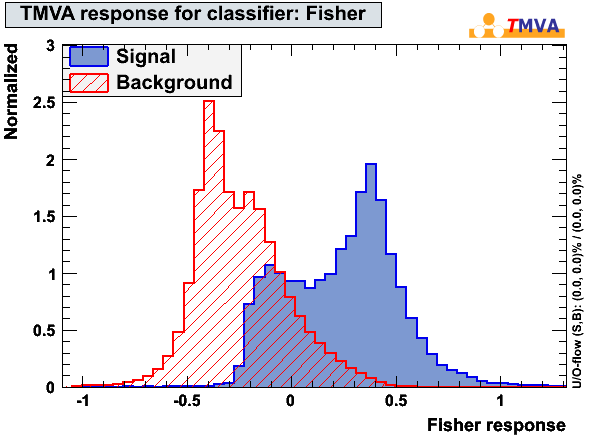
\includegraphics[width=1.0\textwidth]{images/mva_Fisher.png}
\end{minipage}
 \hfill
\begin{minipage}{8.0cm}
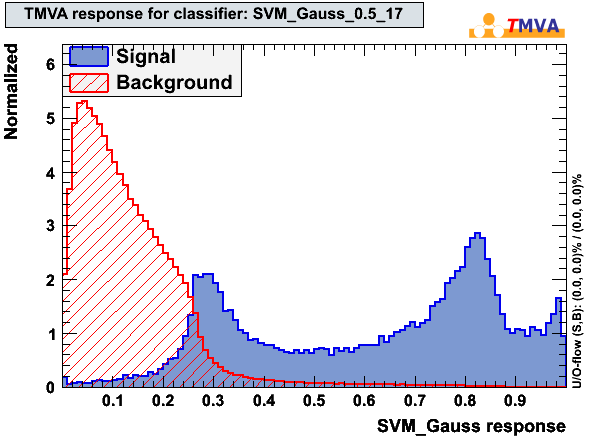
\includegraphics[width=1.0\textwidth]{images/mk_svm_gauss2.png}

%  \label{fig:mkSvmGauss2}
%\end{minipage}


\end{minipage}
%\begin{minipage}{3.0cm}
\caption{\label{fig:fishersvm}TMVA response to Fisher discriminant and 
the output of the SVM classifier with Gaussian kernel.}
%\end{minipage}
\end{figure}

%\begin{figure}[h]
%\begin{center}

%\caption{\label{fig:fisher}TMVA response to Fisher discriminant.}
%\caption{\label{fig:fisher}TMVA response to Fisher discriminant.}
%\end{center}
%\end{figure}

%\begin{figure}[h]
%\begin{center}
%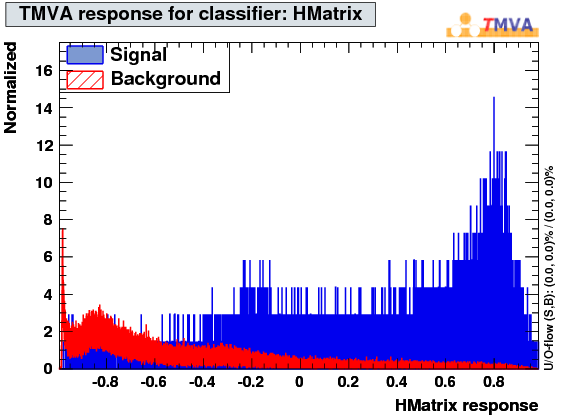
\includegraphics[width=0.8\textwidth]{images/mva_HMatrix.png}
%\caption{\label{fig:hmatrix}TMVA response to H-Matrix discriminant}
%\end{center}
%\end{figure}


\subsection{Boosted Decision Trees}
Recently, the Boosted Decision Trees (BDTs) have been advocated as an alternative to 
artificial neural networks for particle identification~\cite{bdt}.

The BDT method is based on binary decision trees. 
Repeated yes/no decisions are made on the variable with the
best separation power until the subsamples become small or until the
subsamples are declared as signal or background. The variable
phase-space is hence divided into a large number of hypercubes, which is
why BDT is effective for both with linear and non-linear
samples.
%Because the splitting is always based on the variable with
%best separation, variables with small separation power can be input to
%the method without risking loss of performance.

In order to make the decision trees robust against statistical
fluctuations of the training sample, boosting, i.e. reweighting, is
applied to the training sample. After each reweighting, a new decision
tree is constructed. 
The boosting thus combines iteratively many weak classifiers or hypotheses 
into a single stronger rule called the combined hypothesis \cite{bdt}.

The outcome of a tested event is carried out
by evaluating the decisions of typically hundreds of
trees. Overtraining is countered by pruning nodes with insignificant
separation. 


The BDT method was evaluated with a set of 400 trees. Increasing the
tree number was found not to yield significant improvement. The number
of cuts was set to 20 and the pruning strength
parameter of 4.0 was chosen. An example of a decision tree generated
with these parameters is shown in Fig.~\ref{fig:bdt}. The signal efficiency was
found to be 1.12$\pm$0.05\% at background rejection of 10$^5$.
Decorrelation and principal component analysis were tried out for the
input variables, but they were found to yield only minimal changes in
the signal efficiency for the evaluated background rejection points.

% Figure of a decision tree to be added here



\begin{figure}[h]
 \begin{minipage}{9.0cm}
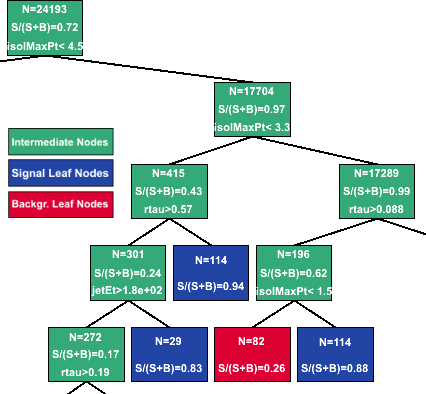
\includegraphics[width=1.0\textwidth]{images/bdt.png}
\end{minipage}
% \hfill
%\begin{minipage}{7.0cm}
%\end{minipage}
\begin{minipage}{6.0cm}
\caption{An example of a boosted decision trees.}
  \label{fig:bdt}
\end{minipage}
\end{figure}


\subsection{Support Vector Machine}
The Support Vector Machine (SVM) learning algorithm is a recent alternative to MVA methods.
One of the first applications in HEP was the classification problem 
of signal/background discrimination in the $t\bar{t}$ dilepton channel~\cite{svmtt}.


The SVM maps the input vectors into the feature space through some
non-linear mapping. 
In this space an optimal hyperplane is constructed  and evaluated by using kernel function.
%${\rm K(u,v)}$~\cite{svmintro}. 

Potential advantages of the SVM method compared to the ANN method
include the existence of only few user chosen parameters, ability to find global minimum, and
correspondence to a linear method which makes the SVM theoretically easy to analyse.

For $\tau$ tagging the SVM was trained with 4k signal jets and 32k background jets.
The SVM training time  scales as O($n^2$), where $n$ is the number of events in the training sample,
so data sample size was kept small for this discriminator.

The SVM parameter space $(\sigma, C)$
was optimized with 2-dimensional grid scan,  
and evaluation for each point was run in parallel in a Linux cluster.

The signal efficiency was found to be 5.6$\pm$0.1\% at background rejection of 10$^5$.
Figures 
%\ref{fig:mkSvmGauss2}
\ref{fig:fishersvm}
 and \ref{fig:mkSvmParallels} demonstrate the TMVA output of the SVM classifier
with Gaussian kernel.

%and in practice training took roughly one hour. 
%\begin{itemize}
%\item Training 4000 signal jets, 32000 background jets

%  \end{itemize}
%\item Results
%  \begin{itemize}
%  \item Background 1
%    \begin{itemize}
%    \item $10^{-5}$ bkg eff: $5.68\pm 0.12\;\%$
%    \item $10^{-6}$ bkg eff: $1.66\pm 0.06\;\%$
%    \end{itemize}
%  \item Background 2
%    \begin{itemize}
%    \item $10^{-5}$ bkg eff: $5.49\pm 0.12\;\%$
%    \item $10^{-6}$ bkg eff: $1.80\pm 0.07\;\%$
%    \end{itemize}
%
%  \end{itemize}
%\end{itemize}

 
%\begin{figure}[h]
% \begin{minipage}{7.0cm}
%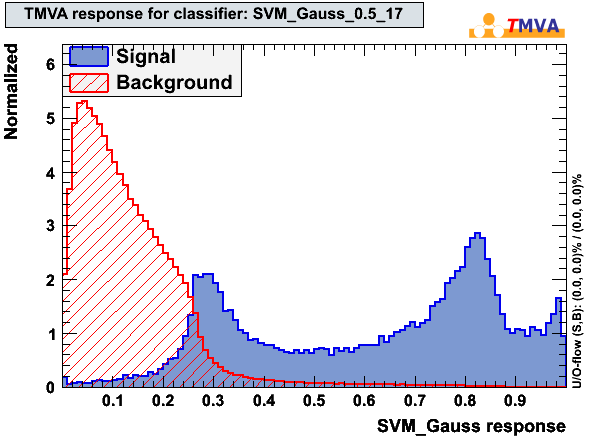
\includegraphics[width=0.8\textwidth]{images/mk_svm_gauss2.png}
%\end{minipage}
% \hfill
%\begin{minipage}{7.0cm}

%\end{minipage}
%\begin{minipage}{3.0cm}
%\caption{The output of the SVM classifier with Gaussian kernel.}
%  \label{fig:mkSvmGauss2}
%\end{minipage}

%\end{figure}


\begin{figure}[h]
\begin{center}
%\includegraphics[width=21pc]{poster/images/.png}\hspace{2pc}%
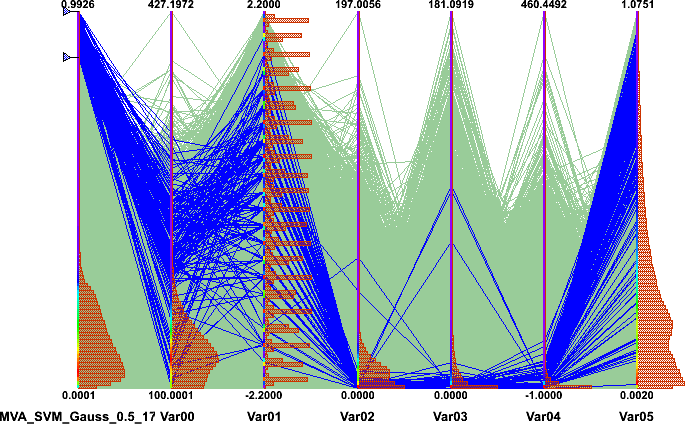
\includegraphics[width=1.0\textwidth]{images/svm_parallels2.png}
%\begin{minipage}[b]{14pc}
  \caption{TMVA plot for parallel coordinates. 
Poorly classified background events with value 0.9-1.0 are selected from vertical histogram on left. 
In this kind of plot each line going through variables,
as explained in Table~\ref{tab:variables}, 
represent on event, possibly giving insight to better variable selection.
%Variables {\tt jetEt, jeteta, isolMaxPt, ecalIsolEt, hcalRatio}, and {\tt rtau} 
%are represented with Var00-Var05 in the figure.

}
  \label{fig:mkSvmParallels}

%\end{minipage}
\end{center}
\end{figure}


\subsection{Neural Networks}
An interesting study related to our $\tau$ tagging is given in~\cite{tauneural}, 
where a artificial network network (ANN ) was trained to choose the polarity of $\tau$ particles from they decay angles.
It was shown that $\tau$ helicity found by the ANN 
approximated well the optimal Bayesian classifier.

%obtain correct polarization for the $\tau$ lepton and
%its decay products~


%Results for MLP discriminator are shown for {\tt jetEt} transformation $log({\rm E}_{\rm T})$ and 
%Principal Component Analysis ({\tt  VarTransform=PCA}).


Of the three Multilayer Perceptrons (MLP) implementations supported by TMVA
{\tt TMVA::Types::kMLP} was selected.
Data for 6-15-1 MLP configuration with neurons of sigmoid type was trained 1k cycles using
10k signal jets and 40k background jets. 
Rest of the data was used for testing (30k signal and 2230k background jets).
A ROOT TMVA script for these settings can be written as follows:
 
\begin{verbatim}
NSigTrain=10000:NBkgTrain=40000:SplitMode=Random:NormMode=NumEvents:!V

MLP_v0  H:!V:!Normalise:NeuronType=sigmoid:NCycles=1000:HiddenLayers=N+9,N:
TestRate=5:VarTransform=PCA
\end{verbatim}

In addition to variable transformation $log({\rm E}_{\rm T})$ 
Principal Component Analysis, PCA, (see {\tt  VarTransform=PCA} above) was found to improve 
classification power.
In our $\tau$ tagging problem the PCA method simply performs a rotation 
in the 6-dimensional orthogonal parameter space to a new coordinate system whose unit vectors
are the eigenvectors of the system. 


Systematic uncertainty was estimated by repeating the full analysis with independent background data.
Convergence of the neural network training and 
background rejection vs. signal efficiency plot  for test data are shown in Fig.~\ref{fig:nn}.

The signal efficiency for MLP discriminator was found to be  6.5$\pm$0.1\% at background rejection of 10$^5$.
\begin{figure}[h]
 \begin{minipage}{8.1cm}
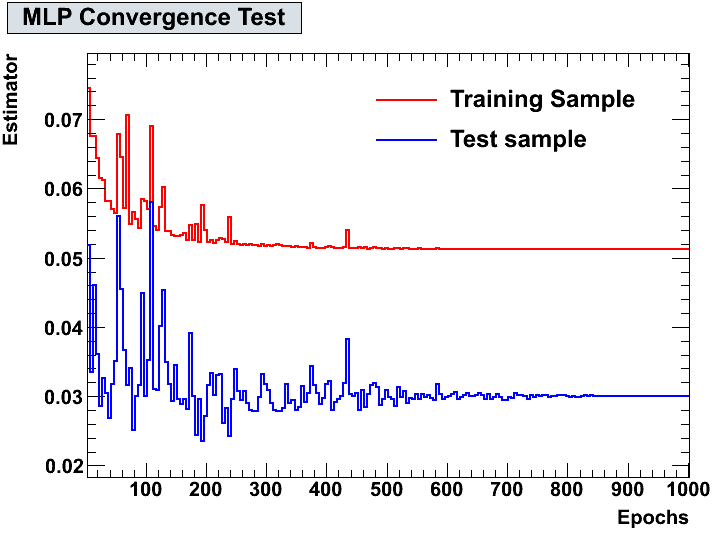
\includegraphics[width=1.0\textwidth]{images/MLPConvergenceTest.png}
\end{minipage}
 \hfill
\begin{minipage}{8.1cm}

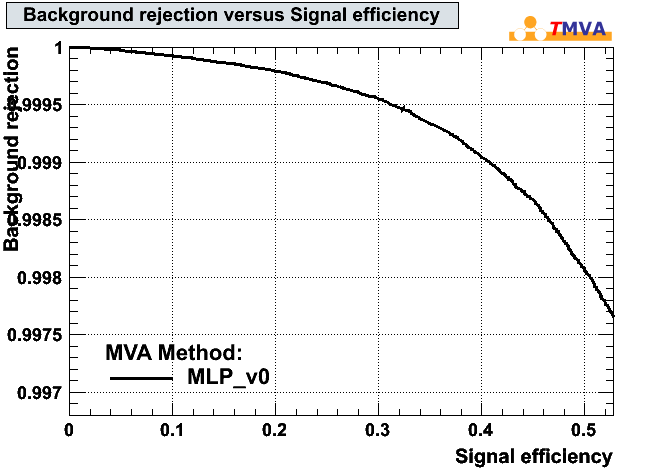
\includegraphics[width=1.0\textwidth]{images/roc.png}
\end{minipage}
%\begin{minipage}{3.0cm}
\caption{Evolution of training and validation errors of ANN during 1000 training cycles and 
background rejection vs. signal efficiency.}
%\end{minipage}
\label{fig:nn}
\end{figure}

\subsection{Summary of results}
Performance of various TMVA discriminators for the ideal $\tau$ tagging problem
are summarised in Table~\ref{table:eff}.

Overall discrimination performance of selected TMVA classifiers are
demonstrated with Receiver Operating Characteristics (ROC) curves in
Fig.~\ref{fig:roc}.

\begin{table}[h]
\caption{\label{table:eff}Summary of performance of various 
TMVA discriminators for the ideal $\tau$ tagging problem.}
\begin{center}
%\begin{tabular}{l*{2}{l}r}
\begin{tabular}{l*{2}{l}{l}r}
\br
Discriminator & Signal efficiency (\%) & \\
              & for background efficiency & \\
              &  $10^{-5}$    & $10^{-6}$              \\
\mr
Fisher   & 3.5$\pm$0.9 (stat) $\pm$ 0.0 (syst)   & 1.6 $\pm$ 0.1 $\pm$ 0.1  \\
BDT      & 1.12$\pm$0.05  $\pm$ 0.1 & NN$\pm$NN $\pm$ 0.1\\
SVM      & 5.6$\pm$0.1  $\pm$ 0.1   & 1.7$\pm$0.1 $\pm$ 0.1   \\
MLP      & 6.5$\pm$0.1  $\pm$ 0.2   & 2.2$\pm$0.1 $\pm$ 0.2   \\
\br
\end{tabular}
\end{center}
\end{table}
%H-Matrix & 1.1$\pm$0.5 (stat.) $\pm$ 0.1 (syst.)  & NN $\pm$ NN $\pm$ NN    \\

\begin{figure}[h]
 \begin{minipage}{8.0cm}
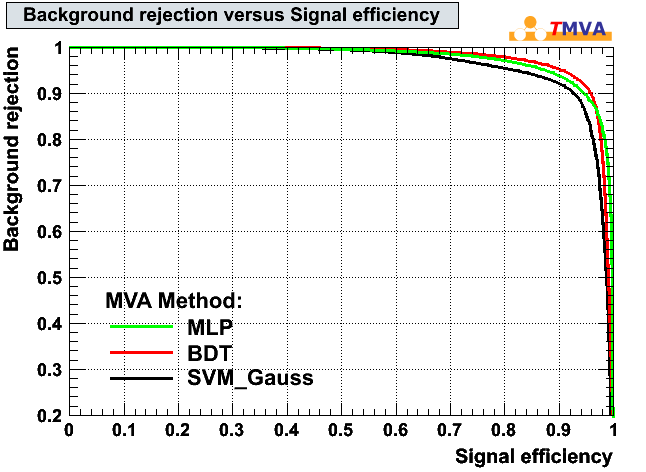
\includegraphics[width=1.0\textwidth]{images/mk_roc.png}
\end{minipage}
 \hfill
\begin{minipage}{8.0cm}
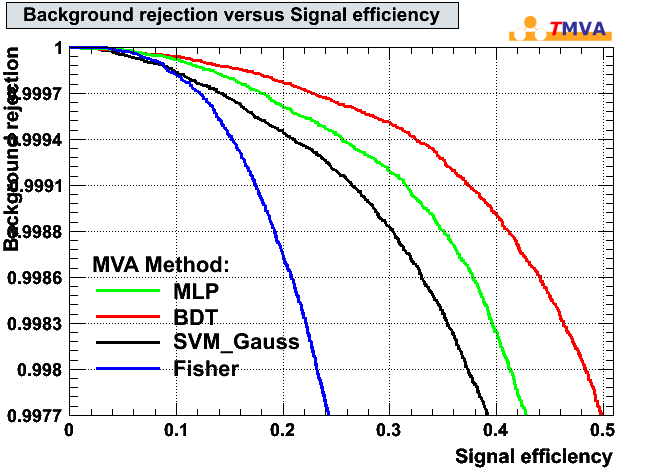
\includegraphics[width=1.0\textwidth]{images/mk_roc_zoomed.png}
\end{minipage}
%\begin{minipage}{3.0cm}

\caption{Overall discrimination performance of selected TMVA classifiers.}
%Receiver Operating Characteristics (ROC) Curve
%\end{minipage}
\label{fig:roc}
\end{figure}

\section{Conclusion}
The usage of TMVA package in ROOT for $\tau$ identification in the
framework of a charged Higgs boson study was discussed from the
point of view of a user. It was observed, that the TMVA package has
matured since CHEP'07 and it is now fully integrated to ROOT. It also
provides an interface for adding new classifiers.

Some customisation was needed to evaluate the study case in the TMVA
framework. The multivariate data-analysis techniques were found to
be promising in $\tau$ identification.
At $10^{-5}$ background efficiency, TMVA classifiers were found to
yield 1.1--6,5~\% signal efficiency. 
Several methods give results comparable, suggesting that they close to the Bayesian limit
of achievable ideal separation.

Areas where our approach can be improved have been identified.
%(e.g. using additional variables, and yet unused classifiers available in TMVA), 
One possibility would be to use more fundamental set of variables, 
instead of those chosen in this study, 
such as the momenta ${\rm p_x}$, ${\rm p_y}$, ${\rm p_z}$ of the final state particles. 
This kind of jet analysis based on neural networks has been shown to simulate a sophisticated 
jet algorithm ${\rm k_\bot}$~\cite{jetanalysis}.

%Additional research on $\tau$ identification is planned.
% \ack %command \ack sets the acknowledgments heading as an unnumbered section.


\appendix % The command \appendix" is used to signify the start of the appendixes.
\section{Customisation of TMVA event evaluation}

Customisation of TMVA for simulated $\tau$ tagging events is demonstrated in 
Listing~\ref{listing:eventcode} and corresponding example from TMVA run is
shown in Listing~\ref{listing:log}.


\lstset{%emph={If,For,Else},emphstyle=\underbar,
language=python,
keywordstyle=\underbar,
caption=Pseudocode for the event evaluation.,
breaklines=true,
stepnumber=99999,  %trick to remove line numbering
showlines=false,
label=listing:eventcode
}
\lstinputlisting{eventcode.txt}

%\newpage

\lstset{emph={Jog},emphstyle=\underbar,
language=,
caption=Example listing from TMVA analysis showing customisations done.,
breaklines=true,
stepnumber=99999,  %trick to remove line numbering
showlines=false,
label=listing:log
}
\lstinputlisting{log.txt}


%\begin{equation}
%time= money
%\end{equation}

%To obtain a simple heading of `Appendix' use the code \verb"\section*{Appendix}". 
%If it contains numbered equations, figures or tables the command \verb"\appendix" should
%precede it and \verb"\setcounter{section}{1}" must follow it. 


\section*{References}

\begin{thebibliography}{9}

%\bibitem{incl} A. Boudard et al., \emph{Intranuclear cascade model for
%    a comprehensive description of spallation reaction data}, Phys.
%  Rev. C66 (2002) 044615
%\bibitem{g4} \emph{Geant4 collaboration website} \\ {\tt http://\-cern.ch/\-geant4}
%\bibitem{pk08bProceedings}
%A. Heikkinen, P. Kaitaniemi, and A. Boudard,
%{\em Implementation of INCL4 cascade and ABLA evaporation codes in Geant4},
%Journal of Physics: Conference Series 119 (2008) 032024, 
%{\sf [doi:10.1088/1742-6596/119/3/032024]}

\bibitem{statlearn} J.~Zimmermann and C.~Kiesling,
\emph{Statistical learning methods in high-energy and astrophysics analysis},
Nucl. Instr. and Meth. A 534 (2004) 204-210

\bibitem{chep07tmva} T.~Lampen {\em et. al.}, \emph{Testing TMVA software in b-tagging 
                  for the search of MSSM Higgs bosons at the LHC},
CHEP’07 proceedings, Journal of Physics: Conference Series 119 (2008) 032028

\bibitem{ptdrII} {CMS Collaboration}, \emph{{CMS} Physics Technical Design Report, Volume {II}:
             Physics Performance}, J. Phys. G: Nucl. Part. Phys. 34 (2007) 995-1579

\bibitem{pythia} T. Sj\"ostrand et al., \emph{High-Energy-Physics
  Event Generation with {PYTHIA} 6.1}, Comp. Phys. Comm. 135 (2001) 238-259

\bibitem{tauola} S.~Jadach et al., \emph{The $\tau$ decay library
  {TAUOLA}: Version 2.4}, Comp. Phys. Comm. 76 (1993) 361-380

\bibitem{maxsusy} M.~Carena et al. \emph{Suggestions for Improved Benchmark Scenarios for Higgs-Boson Searches at LEP2}, 
{\tt arXiv:hep-ph/9912223} %\href{http://arxiv.org/pdf/hep-ph/9912223}{arXiv:hep-ph/9912223}

\bibitem{taupolarization} D.~P.~Roy, \emph{The hadronic tau decay signature of a heavy charged Higgs
              boson at {LHC}}, Phys. Lett. B 459 (1999) 607-614

\bibitem{tautagging} S.~Gennai et al., \emph{Tau jet reconstruction
  and tagging with {CMS}}, Eur. Phys. Jour. C 46 (2006) 1-21


 in analyses of several HEP experiments, for instance in BaBar \cite{fisherbabar} and
Belle \cite{fisherbelle}

\bibitem{fisherbabar} {\tt hep-ex/0105018} (2001)

\bibitem{fisherbelle} Phys. Lett. B 517, 309-318 (2001)

\bibitem{tmvasite} TMVA documentation at {\tt http://tmva.sourceforge.net}

\bibitem{bdt} B.~Roe et al. \emph{Boosted Decision Trees as an 
Alternative to Artificial Neural Networks for Particle Identification},
{\tt arXiv:physics/0408124}

\bibitem{svmtt} A.~Vaiciulis, \emph{Support vector machines in analysis of top quark production},
Nucl. Instr. and Meth. A 502 (2003) 492-494

\bibitem{svmintro}N.~Cristianini and J.~Shawe-Taylor, \emph{An Introduction to Support Vector Machines},
Cambridge University Press, UK 2000

\bibitem{tauneural} L.~Garrido and V.~Gaitan, 
\emph{Use of Neural Nets to Measure the Tau Polarization and its Bayesian Interpretation},
UAB-LFAE-91-04, April, 1991 Universitat Atonoma de Barcelona

\bibitem{tmvaPhystat} F.~Tegenfeldt, \emph{TMVA - Toolkit for multivariate
data analysis with ROOT}, presentation at PHYSTAT-LHC Workshop on
Statistical Issues for LHC Physics, June 27--29 2007.

\bibitem{jetanalysis} P.~De Felice at al., 
\emph{Jet analysis by neural networks in high energy hadron-hadron collisions},
Physics Letters B 354 (1995) 473-480

%\bibitem{htau} {CMS Collaboration}, \emph{{CMS} Physics Technical Design Report, Volume {II}:
%             Physics Performance}, J. Phys. G: Nucl. Part. Phys. 34 (2007) 995-1579
%\bibitem{abla} J. Benlliure et al., \emph{Calculated nuclide
%    production yields in relativistic collisions of fissile nuclei},
%  Nuc. Phys. A628 (1998) 458
%\bibitem{abla1} J. J. Gaimard et al., \emph{},
%  Nuc. Phys. A531 (1991) 709
%\bibitem{abla2} A. R. Junghans et al., \emph{},
%  Nuc. Phys. A629 (1998) 635
%\bibitem{gsifragments} T. Enqvist et al. \emph{},
%  Nucl. Phys. A686 (2001) 481
%\bibitem{g4incl} \emph{Geant4 Physics Reference Manual: INCL~4.2 Cascade and ABLA~V3 Evaporation with Fission} 
%\\ {\tt http://geant4.web.cern.ch/\-geant4/\-UserDocumentation/\-UsersGuides/\-PhysicsReferenceManual/\-html/\-node185.html}

%\bibitem{data} X.Ledoux et al., \emph{Spallation Neutron Production by
%  0.8, 1.2, and 1.6 GeV Protons on Pb Targets} Phys. Rev. Lett. 82
%  (1999)

%\item Strite S and Morkoc H 1992 {\it J. Vac. Sci. Technol.} B {\bf 10} 1237 
\end{thebibliography}


\end{document}



